\documentclass[letterpaper,man,natbib,noextraspace,floatsintext,longtable]{apa6}  

\usepackage[english]{babel}
\usepackage[utf8x]{inputenc}
\usepackage{amsmath}
\usepackage{graphicx}
\usepackage{booktabs}             % fancy latex tables
\usepackage[export]{adjustbox}    % center wide tables on page
\usepackage{setspace}             % adjust caption linespacing 
\usepackage{multibib}             % references in supplement
\usepackage{hyperref}             % manage hyperlink colors

% override apa6 section headers
% https://tex.stackexchange.com/questions/125537/how-to-modify-subsubsection-header-apa6-cls
\makeatletter
\renewcommand{\subsubsection}{\@startsection{subsubsection}{3}
  {\z@}%
  {\b@level@two@skip}{\e@level@two@skip}%
  {\normalfont\normalsize\bfseries}}
\makeatother

% center contents of longtable
\usepackage{array}
\newcolumntype{P}[1]{>{\centering\arraybackslash}p{#1}}

% setup supplementary references
\newcites{SM}{Supplementary references}

% decrease size of references (lol)
\renewcommand*{\bibfont}{\small}

% change hyperlink colors
\hypersetup{
    colorlinks=true,
    linkcolor=blue,
    filecolor=magenta,      
    urlcolor=cyan,
    citecolor=blue
}

\title{Confirmatory factor analysis of the Maltreatment and Abuse Chronology of Exposure (MACE) scale: Evidence for essential unidimensionality}
\shorttitle{Confirmatory factor analysis of the MACE}
\author{Samuel Zorowitz$^1$, Lauri Tuominen$^{2}$}
\affiliation{$^1$Princeton Neuroscience Institute, Princeton University, USA\\$^2$The Royal’s Institute of Mental Health Research, University of Ottawa, Canada}

\abstract{

\noindent \textbf{Background}: The Maltreatment and Abuse Chronology of Exposure (MACE) scale is a retrospective self-report scale that measures 10 distinct types of childhood maltreatment. Despite its increasing use, the factor structure of the MACE has not been thoroughly investigated. As such, the viability of the MACE total and subscale scores are uncertain. The aim of the present study was to investigate the factor structure of the MACE and to quantify the reliability of its total and subscale scores. 

{\begin{spacing}{1.25} \hfill \\ \end{spacing}}

\noindent \textbf{Methods}: We evaluated a series of confirmatory item factor models fit to the responses of two independent samples of participants (N=1051 \& N=582) who completed the MACE. The models included hierarchical (bifactor) models. We used model-based indices to estimate the reliability of the MACE total and subscale scores, and to quantify the essential unidimensionality of the scale.

{\begin{spacing}{1.25} \hfill \\ \end{spacing}}

\noindent \textbf{Results}: We found the MACE total score was a reliable and valid measure of overall childhood maltreatment. In contrast, although MACE subscale scores exhibited adequate reliability, we found that the vast majority of reliable variance in these scores reflected general maltreatment and not any particular type of maltreatment as intended. We also found that the MACE is essentially unidimensional, and exhibits evidence of differential item functioning by gender.

{\begin{spacing}{1.25} \hfill \\ \end{spacing}}

\noindent \textbf{Conclusions}: Our results provide support for a one-factor structure of the MACE, as well as continued use of the MACE total score. Our results caution against the use of MACE subscale scores, which have little practical use given that they provide little unique or reliable information above and beyond the total score.

\hfill \break

}

\keywords{child maltreatment, reliability, item response theory, bifactor model}

\authornote{This research was funded by the Royal's Emerging Research Innovators in Mental Health program at the University of Ottawa Institute of Mental Health Research and a National Science Foundation Graduate Research Fellowship. The authors wish to thank Dr. Robyn McQuaid for thoughtful feedback on this manuscript. The authors have no conflicts of interest to declare.}

\begin{document}

\maketitle

\section{Introduction}

Childhood maltreatment is an unfortunately common experience for children around the world \citep{stoltenborgh2015prevalence}. It is a risk factor for multiple poor outcomes later in life including the development of mental illness \citep{kessler2010childhood}, cognitive impairment \citep{su2019does}, and poor physical health \citep{wegman2009meta}. Childhood maltreatment also predicts worse treatment outcomes for several psychiatric disorders \citep{nanni2012childhood, thomas2019childhood}. Thus, the reliable and valid assessment of childhood maltreatment is an important research goal in order to refine our understanding of the link between maltreatment and health outcomes; augment treatment strategies for victims of childhood maltreatment; and ultimately design better interventions to prevent maltreatment in the first place. 

There already exist many measures of childhood abuse and maltreatment for researchers to choose from \citep{saini2019systematic}. One recently developed measure, the Maltreatment and Abuse Chronology of Exposure scale (MACE; \citealt{teicher2015maltreatment}), has a number of notable advantages. First, the MACE is a 52-item retrospective self-report scale composed of 10 subscales, each of which measures a unique type of childhood maltreatment. The content of six of these subscales overlap with other childhood maltreatment scales (e.g. physical abuse, neglect), whereas the remaining four are less commonly represented in other scales (e.g. peer victimization, witnessing domestic violence). Second, the items in the MACE were carefully selected to measure maltreatment of increasing severity in order to finely differentiate people with differing exposure levels. Third, the MACE also asks for the onset and duration of maltreatment experiences, which is necessary for investigating how the timing of abuse shapes development. Finally, the MACE was originally developed to provide two measures: a total score (number of overall maltreatment experiences) and a multiplicity score (number of types of maltreatment experienced). These scores have excellent temporal stability, convergent validity with other childhood maltreatment scales, and good predictive validity for a multitude of psychiatric symptoms \citep{teicher2015maltreatment}. For these reasons, the MACE has been included as among the best measures of childhood maltreatment currently available \citep{saini2019systematic, georgieva2022systematic}.

In recent years, there have been calls for childhood maltreatment research to move away from the cumulative risk framework \citep{evans2013cumulative} --- which focuses only on the number of adverse experiences --- towards a dimensional approach, which emphasizes how distinct types of maltreatment uniquely shape developmental trajectories \citep{mclaughlin2016beyond, belsky2012beyond}. In response, some researchers have begun to use the MACE to make new indices of maltreatment in lieu of, or in addition to, the total and multiplicity scores. For example, some researchers have used all 10 MACE subscale scores to study the unique contributions of each type of maltreatment to the development of psychopathology \citep{schalinski2015type, gerke2018childhood, schalinski2019early}. Citing a prominent dimensional model of maltreatment \citep{mclaughlin2014childhood}, others have made novel threat and deprivation subscale scores made up of items in the MACE that measure abuse and neglect experiences, respectively \citep{schalinski2018defining, schalinski2019environmental, teicher2018differential}. The psychometric properties of these subscale scores have not been thoroughly investigated.   

A critical challenge in studying the consequences of childhood maltreatment is the high co-occurrence of these adverse experiences. That is, children who have experienced any single type of maltreatment are likely to have experienced multiple other types \citep{dong2004interrelatedness, herrenkohl2009assessing, kessler2010childhood}. As such, isolating the unique contribution of one type of maltreatment to an outcome is difficult insofar as any one type of adversity is likely confounded with overall maltreatment. Concretely, this means that researchers intending to study the sequela of particular types of maltreatment using subscale scores need to verify that those scores actually reflect a construct unique from overall maltreatment, lest they risk drawing spurious conclusions.

Bifactor models, a type of hierarchical factor model, are well-suited for addressing this issue \citep{bornovalova2020appropriate}. They assume that the covariation in responses to a set of items can be accounted for by a \emph{general} factor, reflecting shared variance across all items, and one or more \emph{specific} factors, reflecting additional shared variance among subsets of items \citep{Reise2012-ql}. Crucially, bifactor models can be used to calculate model-based reliability statistics, including the omega hierarchical ($\omega_h$) and omega subscale ($\omega_s$) indices \citep{reise2013scoring}, which respectively measure the proportion of variance in total and subscale scores attributable to the general factor and specific factors. Applied to the MACE, these indices can help determine if subscale scores measuring particular types of maltreatment are interpretable as such, or if they instead principally reflect overall maltreatment. In addition, bifactor models permit the calculation of other useful indices like the explained common variance (ECV; \citealt{sijtsma2009use}), which measures what fraction of the total reliable variance in a scale can be attributed to a general factor. Applied to the MACE, the ECV can quantify the degree to which the MACE is essentially unidimensional (i.e. summarizable by a one-factor model). 

The overarching aim of the present study was to investigate the factor structure of the MACE, which has received little previous study to date \citep{saini2019systematic}. To do so, we fit and evaluated a series of confirmatory item factor models to the responses from two independent samples of participants who completed the MACE. The primary goal of our analyses was to quantify the reliability of the MACE total and subscale scores, and to determine whether the latter would provide unique information above and beyond the total score. A secondary goal was to examine the dimensionality of the MACE; that is, to determine whether responses on the MACE are best-explained by a hierarchical structure with 10 factors (one per subscale) or by a more parsimonious factor structure. All data and analysis materials are publicly available at: \url{https://github.com/szorowi1/mace-irt}.

\section{Methods}

\subsection{Participants}

The participants in the current study (N=1633 total) belonged to one of two samples. The first sample of participants (N=1051) are from the original development of the MACE \citep{teicher2015maltreatment}. The full recruitment details for this sample have been reported elsewhere \citep{teicher2015maltreatment}. Briefly, these participants were recruited from the greater Boston area between 2010 and 2013. Inclusion criteria included being medically healthy, unmedicated, and between 18–25 years of age. This sample will hereafter be referred to as the \textit{original} sample. 

The second sample of participants (N=687) were recruited from the Prolific Academic platform (\url{https://www.prolific.co}) to participate in an online experiment in August -- October, 2021. Of these, N=582 were retained for analysis (see Exclusion Criteria below). Participants were eligible for participation if they were 18 years or older and currently resided in the United States or Canada. Participants received monetary compensation for their time (rate: \$12 USD/hr). This study was approved by the Institutional Review Board of the University of Ottawa (\#2021003), and all participants provided informed consent. This sample will hereafter be referred to as the \textit{replication} sample. 

\begin{table}[t!]
    \centering
    \begin{tabular*}{\textwidth}{lccc}
    \toprule
    Variable & Original (N=1051) & Replication (N=582) & p-value \\
    \midrule
    \textbf{Gender}, N (\%)                & & & p < 0.001 \\
    \hspace{1em} Women                     & 670 (63.7\%) & 310 (53.3\%) & \\
    \hspace{1em} Men                       & 381 (36.3\%) & 258 (44.3\%) & \\
    \hspace{1em} Transgender or NB         &   0  (0.0\%) &   9  (1.5\%) & \\
    \hspace{1em} Rather not say            &   0  (0.0\%) &   5  (0.9\%) & \\
    \midrule
    \textbf{Age}, yrs                      & & & p < 0.001 \\
    \hspace{1em} Mean (range)              & 23.1 (18 -- 27) & 30.2 (18 -- 80) & \\
    \midrule
    \textbf{Ethnicity}, N (\%)             & & & p = 0.214 \\
    \hspace{1em} Not Hispanic or Latino    & 963 (91.6\%) & 518 (89.0\%) & \\
    \hspace{1em} Hispanic or Latino        &  84  (8.0\%) &  57  (9.8\%) & \\
    \hspace{1em} Rather not say            &   4  (0.4\%) &   7  (1.2\%) & \\
    \midrule
    \textbf{Race}, N (\%)                  & & & p = 0.677 \\
    \hspace{1em} White                     & 806 (76.7\%) & 441 (75.8\%) & \\ 
    \hspace{1em} Asian                     & 103  (9.8\%) &  65 (11.2\%) & \\
    \hspace{1em} Black or African American &  81  (7.7\%) &  31  (5.3\%) & \\
    \hspace{1em} Other                     &  61  (5.8\%) &  28  (4.8\%) & \\
    \hspace{1em} Rather not say            &   0  (0.0\%) &  17  (2.9\%) & \\
    \bottomrule
    \end{tabular*}
    \caption{\normalfont Demographics of the two samples included in this study. The original sample was recruited and reported by \cite{teicher2015maltreatment}. The replication sample was recruited by the current authors for the purposes of this study.}
    \label{tab:demographics}
\end{table}

The demographics of the two samples are summarized in Table \ref{tab:demographics}. The majority of participants in both samples identified as women, though the original sample was composed of proportionally more woman than the replication sample ($z$ = 4.142, $p$ < 0.001). Participants in the original sample were also younger on average ($t$ = -19.313, $p$ < 0.001). The majority of participants in both samples identified as White and not as Hispanic or Latino. The proportion of participants identifying as White was not significantly different across samples ($z = 0.417$, $p = 0.677$), nor was the proportion of participants identifying as Hispanic or Latino ($z$ = -1.241, $p$ = 0.214).

\subsection{Measures}

All participants completed the 52-item version of the MACE \citep{teicher2015maltreatment}. The MACE is a retrospective self-report scale that measures 10 unique types of childhood maltreatment (i.e. parental verbal abuse, physical abuse, nonverbal emotional abuse, sexual abuse, emotional neglect, physical neglect, witnessing violence to siblings, witnessing interparental violence, peer verbal abuse, peer physical abuse). For each item, participants endorse whether they ever experienced a particular event during childhood (e.g. ``Parents or guardians intentionally pushed, grabbed, shoved, slapped, pinched, punched or kicked you'') and, if so, at what ages (up to age 18). Here we only analyze the dichotomous endorsement responses (Yes = 1, No = 0) and not the chronology data. Six of the 52-items --- evenly divided between the emotional and physical neglect subscales --- are positively valenced and reverse-scored (e.g. ``One or more individuals in your family helped you feel important or special''). For these items we follow the scoring convention set by \cite{teicher2015maltreatment}: a score of 1 is assigned to a response only in the absence of a positive event for all 18 years of childhood. This is in contrast to all other items, where a score of 1 is assigned if maltreatment was experienced in at least one year of childhood.

In both the original and replication samples, participants completed a number of additional self-report symptom measures. We do not include these in our analyses and therefore do not discuss these measures further in the main text. For completeness, we report these secondary self-report measures in the supplementary materials. 

\subsection{Exclusion criteria}

To ensure data quality in the replication sample, we relied on attention checks embedded in the self-report measures to identify and remove participants engaging in careless or insufficient effort responding (\citealt{zorowitz2021inattentive}; see the supplementary materials for the attention checks). The data from N=64 (9.9\%) participants in the replication sample were excluded for failing one or more of these attention checks, leaving the data from N=582 participants for analysis.

\subsection{Differential item functioning}

Prior to analysis, we investigated whether it was appropriate to combine response data from the original and replication samples. We first compared across samples the maltreatment endorsement rates for each item. The Spearman-rank correlation of endorsement rates across samples was large ($\rho$ = 0.951, p < 0.001), indicating excellent correspondence in the relative prevalence of maltreatment types across samples. When we compared the distribution of person-level total scores across samples, however, we found that scores were greater on average in the replication sample than in the original sample ($p_1$ = 0.185, $p_2$ = 0.219, $t$ = -4.611, p < 0.001). 

A mean shift in overall endorsement rates by sample is not necessarily evidence for a violation of measurement invariance. One possibility is that the replication sample had simply experienced more adversity than the original sample. A second is that the differences in the demographic composition of the two samples (e.g. gender, age) explain the differences in endorsement rates. To investigate these possibilities, we tested for uniform differential item functioning (DIF) using logistic regression, in which a participant's response on an item is regressed against their rest score (i.e. their total score for all other items), sample membership, gender, and age.

Using the cutoffs recommended by \cite{hidalgo2014binary}, we identified 11 of 52 items on the MACE with large DIF by study (Figure \ref{fig:dif_study}). These included all six reverse-scored items. We also found an additional 11 items with large DIF by gender (Figure \ref{fig:dif_gender}). Five of these items concerned sexual abuse (endorsed more frequently by women), and another five concerned peer physical abuse (endorsed more frequently by men). We identified no items that exhibited large DIF by age. Given the number of items with DIF by sample membership, we decided to analyze each sample separately.

\subsection{Item response dependence}

Also prior to analysis, we found that the MACE contains a total of 12 item pairs and triplets characterized by response dependence (Table \ref{tab:dependence}). The items in some of these sets are structurally dependent, where a response to one item requires or strongly implies a certain response on the second. For example, a person endorsing item 8 (``Parents or guardians hit you so hard that you received medical attention'') is all but certain to endorse item 7 (``Parents or guardians hit you so hard that it left marks for more than a few minutes''). Other items are dependent by virtue of redundancy. One such example is items 36 (``Peers forced you to engage in sexual activity against your will'') and 37 (``Peers forced you to do things sexually that you did not want to do``); here the same question is asked twice using slightly different language.

Structurally-dependent or redundant items can cause serious problems for item factor models. First, they can inflate the estimates of item discrimination parameters, making items appear more reliable than they actually are \citep{marais2008formalizing}. Second, response dependence can cause overestimation of item loadings on specific factors in bifactor models, making specific factors (and subscores) appear more reliable than they actually are \citep{reise2013applying}. Following \cite{marais2008formalizing}, we therefore combined each set of dependent items into a single polytomous item thereby reducing the MACE from 52 to 39 items in total.

\subsection{Confirmatory item factor models}

To investigate the factor structure of the MACE, we fit a series of four confirmatory item factor models separately to the response data from each sample.\footnote{The suitability of common factor models (CFMs) with reflective indicators for explaining childhood maltreatment data has been contested. For interested readers, we justify our use of CFMs to explain responses to the MACE in the supplement.} The basis of each model is the graded response model for ordered polytomous data \citep{samejima1997graded}. The factor structure for each model is depicted in Figure \ref{fig:models}. The first is a one-factor (undimensional) model where all items load onto a general maltreatment factor (Figure \ref{fig:models}a). The second is a bifactor model where all items load onto a general maltreatment factor and also one of 10 specific factors based on their subscale membership (Figure \ref{fig:models}b). This model will be used to evaluate if the MACE can produce reliable subscale scores for each of the 10 types of maltreatment assessed by the MACE. 

The third model was motivated by a dimensional theory of childhood maltreatment that distinguishes between threat and deprivation experiences as two distinct types of adversity \citep{mclaughlin2014childhood}. To examine this model of the MACE, we initially fit a bifactor model where all items loaded onto a general maltreatment factor, and also a threat or neglect specific factor. However, we observed vanishing item loadings on the threat specific factor. Therefore, we instead fit a bifactor S-1 model \citep{eid2017anomalous} where all items load onto a general maltreatment factor, and only items measuring neglect (i.e. items from the physical and emotional neglect subscales) load onto a specific neglect factor (Figure \ref{fig:models}c). We fit this model to see if the MACE can be used to form neglect subscale scores that are reliable and distinguishable from general maltreatment. 

\begin{figure}[t!]
    \centering
    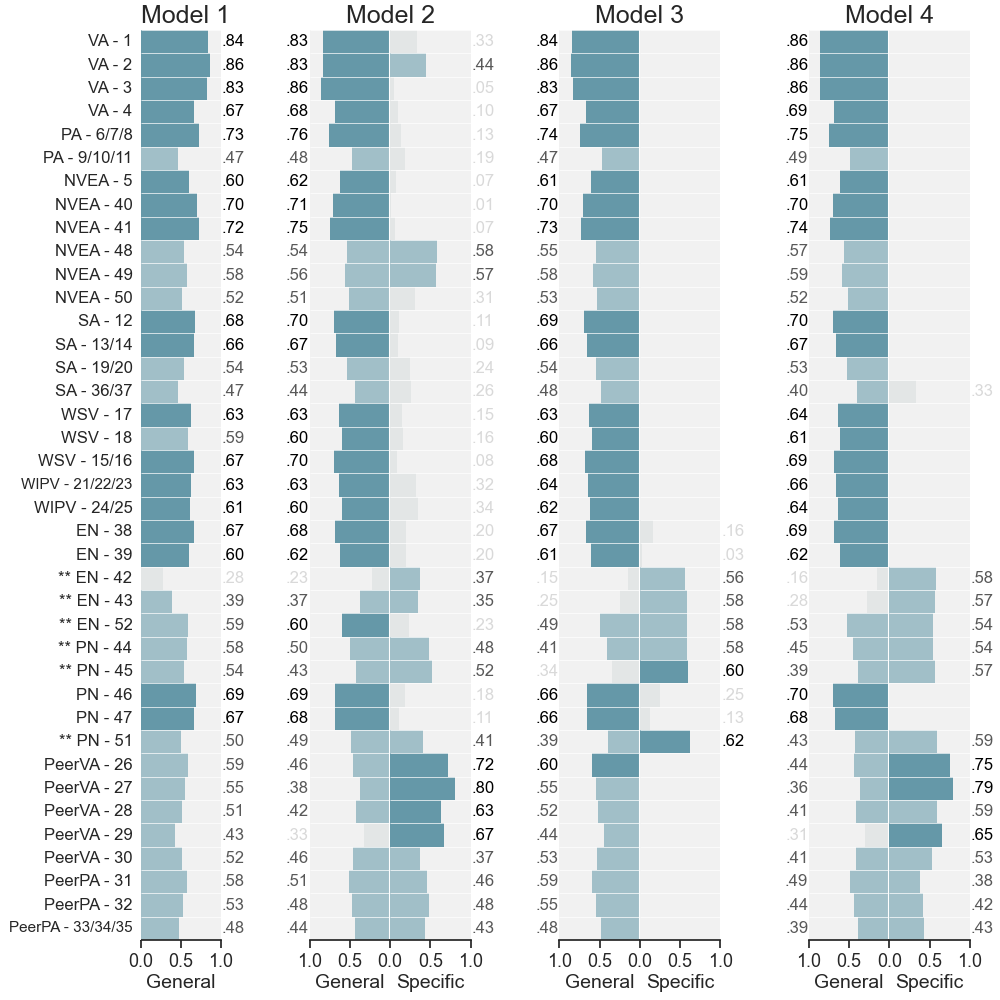
\includegraphics[width=1.1\textwidth,center]{figures/fig01.png}
    \captionsetup{width=1.1\textwidth}
    \caption{\normalfont The structure of the four competing confirmatory factor models of the MACE. (A) One-factor (unidimensional) model. (B) Bifactor model with 10 specific factors (one per MACE subscale). (C) Bifactor S-1 model with 1 specific factor (neglect). (D) Bifactor S-1 model with 2 specific factors (peer victimization, reverse-scored). Notes: G = general maltreatment; VA = verbal abuse; PA = physical abuse; NVEA = nonverbal emotional abuse; SA = sexual abuse; WSV = witnessing sibling vioence; WIPV = witnessing inter-parental violence; EN = emotional neglect; PN = physical neglect; PeerVA = peer verbal abuse; PeerPA = peer physical abuse.}
    \label{fig:models}
\end{figure}

The fourth and final model we fit proposes a more parsimonious structure of the MACE based on the content of its items. Items on the MACE can be categorized according to the source of maltreatment: parents (or other adults in the home) and peers. Thus, we hypothesized there would be two factors underlying responses on the MACE: a primary parental maltreatment factor and a secondary peer victimization factor. From preliminary model fits, we also suspected the presence of a tertiary methods factor affecting the six reverse-scored items. We initially fit a bifactor model in which all items loaded onto a general maltreatment factor and one of three specific factors (parental maltreatment, peer victimization, reverse-scored); however, we observed vanishing loadings on the first specific factor. We instead fit a bifactor S-1 model where all items load onto a general maltreatment factor, and the peer victimization \& reverse-scored items additionally load onto their own specific factors (Figure \ref{fig:models}d). We fit this model in part to test a more parsimonious factor structure of the MACE, and to see if the MACE can be used to form peer victimization subscale scores that are reliable and distinguishable from general maltreatment. 

All confirmatory item factor models were estimated within a Bayesian framework using Hamiltonian Monte Carlo as implemented in Stan (v2.26; \citealt{carpenter2017stan}). For each model, four separate chains with randomized start values each took 3,000 samples from the posterior. The first 2,000 samples from each chain were discarded, so that 4,000 post-warmup samples from the posterior were retained. The $\hat{R}$ values for all parameters were less than 1.01, indicating acceptable convergence between chains, and there were no divergent transitions in any chain. 

\subsection{Goodness of fit \& model comparison}

We relied on multiple indices to judge the fit of the models to the data. First we calculated three traditional goodness-of-fit statistics using the ordinal $M_2$ statistic \citep{cai2013limited}. $M_2$ is asymptotically $\chi^2$-distributed with $\kappa − \nu$ degrees of freedom ($df$), where $\kappa$ is the reduced number of first- and second-order marginal residuals (i.e. $\kappa = n(n + 1)/2$ for $n$ items) and $\nu$ denotes the number of free parameters. To improve the stability of the $M_2$ statistic, the responses to polytomous items were binarized (i.e. any vs. no maltreatment). Using the $M_2$ statistic, we calculated the root mean square error of approximation (RMSEA), comparative fit index (CFI), and Tucker-Lewis index (TLI) for each model fit. Following convention \citep{hu1999cutoff}, the benchmarks for adequate model fit are RMSEA < 0.08, CFI > 0.90, and TLI > 0.90; in turn, the benchmarks for good model fit are RMSEA < 0.05, CFI > 0.95, and TLI > 0.95. 

Given the limitations of SEM-based fit indices for item response models \citep{clark2018model}, we calculated two additional fit indices. First, we used posterior predictive model checking to calculate a $\chi^2_{NC}$ discrepancy measure based on the total score distribution \citep{sinharay2006posterior}. This measure compares the observed and model-predicted proportion of participants at each total score level. Second, to test for local dependence in each pair of items, we calculated Yen's $Q_3$ statistic \citep{yen1984effects} and also the critical $Q_3$-value (i.e. the value above which local dependence is indicated; \citealt{christensen2017critical}). For each model and sample, we simulated 1000 locally independent datasets using the posterior distribution of the model parameters. We then recorded the maximum $Q_3$ value per simulation. The critical $Q_3$-value was defined as the 99th percentile of these max $Q_3$ values. 

The goodness-of-fit of the models was compared using Bayesian leave-one out cross- validation (LOO-CV; \citealt{vehtari2017practical}). The LOO-CV measure quantifies the discrepancy between the model and data while taking into account model complexity. LOO-CV values are presented in deviance scale, i.e. smaller values indicate better fit.

\subsection{Model-based reliability indices}

To evaluate the reliability of the MACE total and subscale scores, we calculated several model-based reliability indices using the factor loadings from the bifactor models. First, we calculated coefficient omega ($\omega$; \citealt{mcdonald2013test}), which quantifies the proportion of reliable score variance attributable to all factors (i.e. both general and specific factors). Next we calculated coefficient omega hierarchical ($\omega_h$) and coefficient omega subscale ($\omega_s$;  \citealt{reise2013scoring}). Whereas $\omega_h$ measures the fraction of total score variance attributable to the general factor, $\omega_s$ measures the fraction of subscale score variance attributable to a specific factor after controlling for the general factor. The values of $\omega_h$/$\omega_s$ facilitate interpretation of total and subscale scores. Values of $\omega_h$ approaching 1 indicate the general factor is the primary source of reliable variance in a total score. When $\omega_h$ > 0.80, the total score may be considered an essentially unidimensional reflection of the general factor \citep{rodriguez2016applying}. Values of $\omega_s$ approaching 1 indicate the specific factor, not the general factor, is the primary source of reliable variance in a subscale score. \cite{canivez2016bifactor} suggested that an acceptable $\omega_s$ value is 0.50 and that >0.70 is desirable. In contrast, values of $\omega_s$ < 0.50 preclude the interpretation of subscale scores as primarily reflecting a specific factor \citep{gignac2013bifactor}. 

To assess the unidimensionality of the MACE, we calculated the explained common variance (ECV; \citealt{sijtsma2009use}) and the proportion of uncontaminated correlations (PUC; \citealt{reise2013multidimensionality}). The ECV is the ratio of the variance explained by the general factor divided by the total common variance of a scale. It thus measures the contribution of the general factor relative to the specific factors. As ECV values approach 1, the general factor loadings of a bifactor model are expected to resemble the item loadings that would be obtained by a one-dimensional model. ECV values greater than 0.70 often indicate a scale is essentially unidimensional \citep{rodriguez2016applying}. In turn, PUC quantifies how many inter-item correlations are accounted for only by the general factor. PUC is an important moderator of the ECV; as PUC increases, ECV is less important for evaluating the risk of bias when fitting a unidimensional model to data with a latent bifactor structure. When PUC > 0.80, there is a low risk of bias when a multi- dimensional scale is treated as unidimensional \citep{reise2013multidimensionality}. We also calculated the relative parameter bias (RPB), which is the difference between an item's loading in a unidimensional model and its corresponding general factor loading in a bifactor model, divided by the general factor loading from the bifactor model. RPB less than 10–15\% is acceptable \citep{muthen1987structural}.

Finally, we calculated the H index to assess the construct replicability of each factor \citep{hancock2001rethinking}. The H index is an estimate of how well a set of items represents a latent factor. H values closer to 1 indicate a well-defined latent factor with item loadings more likely to be stable across studies. In contrast, small H values suggest a poorly defined latent factor where item loadings are liable to change across studies. Because we are presently focused on evaluating the reliability of MACE total and subscale scores, we report the H values below but do not interpret them further.

\subsection{Exploratory factor analysis}

In addition to confirmatory factor analysis, we also performed exploratory factor analysis (EFA) on the response data for each sample separately. The purpose for performing EFA after confirmatory factor analysis was to examine whether any of the hypothesized factor structures emerged from the data with fewer \textit{a priori} restrictions \citep{schmitt2018selecting}. For the sake of brevity, the details and results of the EFA are included in the supplement. 

\section{Results}

\subsection{Goodness-of-fit \& model comparison}

The goodness-of-fit indices for each model and sample are summarized in Table \ref{table:cfa_diagnostics}. According to the traditional indices, each model provided at least an acceptable fit to the data. All RMSEA value were <0.05 and most CFI and TLI values were >0.95. The only exception were for the fits of models 1 and 3 to the original sample data where CFI \& TLI > 0.90. In general, model fits were better for the replication sample data than for the original sample. Furthermore, none of the posterior predictive p-values corresponding to the $\chi^2_{NC}$ discrepancy measure exceeded the critical values indicating that all models were able to reproduce the observed distribution of total scores for each sample.

\begin{table}[t!]
\small
\centering
\begin{adjustbox}{center}
\begin{tabular}{ccccccccccr}
\toprule
Sample & Model & $\chi^2 (df)$ &  RMSEA & CFI & TLI & $\chi^2_{NC}$ (PPP) & $Q3_{\max}$ &  $Q3_{\text{crit}}$ & LOO-CV & \multicolumn{1}{c}{$\Delta$LOO (se)} \\
\midrule
Original & 1 &  1858 (702) &  0.040 &  0.927 &  0.923 &  0.051 (0.230) &  0.589 &  0.239 &  30967.2 &  1748.0 (76.7) \\
& 2 &  1373 (663) &  0.032 &  0.955 &  0.950 &  0.046 (0.356) &  0.573 &  0.300 &  29211.3 & \multicolumn{1}{c}{-} \\
& 3 &  1571 (692) &  0.035 &  0.944 &  0.940 &  0.051 (0.214) &  0.591 &  0.255 &  30531.1 &  1312.0 (68.0) \\
& 4 &  1253 (687) &  0.028 &  0.964 &  0.961 &  0.046 (0.346) &  0.591 &  0.279 &  29219.2 & 7.9 (56.3) \\
\midrule
Replication & 1 &  1086 (702) &  0.031 &  0.954 &  0.952 &  0.065 (0.629) &  0.513 &  0.250 &  19771.6 &  1089.3 (58.4) \\
& 2 &   956 (663) &  0.028 &  0.965 &  0.961 &  0.058 (0.766) &  0.456 &  0.310 &  18706.2 &    24.0 (52.0) \\
& 3 &   881 (692) &  0.022 &  0.977 &  0.976 &  0.062 (0.684) &  0.468 &  0.316 &  19177.7 &   495.5 (45.0) \\
& 4 &   842 (687) &  0.020 &  0.982 &  0.980 &  0.058 (0.756) &  0.437 &  0.318 &  18682.2 & \multicolumn{1}{c}{-} \\
\bottomrule
\end{tabular}
\end{adjustbox}
\captionsetup{width=1\textwidth}
\caption{\normalfont Fit statistics for the confirmatory factor models by sample. LOO-CV values are presented in deviance scale (i.e. smaller values indicate better fit). Notes: RMSEA = root mean square error of approximation; CFI = comparative fit index; TLI = Tucker-Lewis index; PPP = posterior predictive p-value; $Q3_{\max}$ = maximum $Q_3$ value in the sample for the model; $Q3_{\text{crit}}$ = critical $Q_3$ value for the model; LOO-CV = leave-one-out cross-validation.}
\label{table:cfa_diagnostics}
\end{table}

Next we inspected the $Q_3$ indices for evidence of local dependence. For all models and samples, the maximum observed $Q_3$ index was greater than the critical $Q_3$ value. To gauge the extent of local dependence, we visualized the $Q_3$ values for item pairs exceeding the critical value for each model and sample (Figure \ref{fig:local_dependence}). The unidimensional model fits exhibited many locally dependent item pairs --- especially among the peer victimization and reverse-scored items --- suggesting possible underfactorization. By comparison, the remaining three models exhibited many fewer locally-dependent item pairs. Of these pairs, the reasons for dependence were apparent. For example, the residual dependence between items 17 (``Parents made inappropriate sexual comments or suggestions to your sibling'') and 18 (``Parents touched or fondled your sibling in a sexual way'') certainly stems from the fact that these items measure highly similar content. Regardless, the estimated item discrimination parameters for each model fit seldom exceeded the normal range ($\alpha \leq 4$). That is, the level of local dependence present in the models did not cause substantial bias in parameter estimation \citep{edwards2018diagnostic}. Thus, we conclude that all model fits provide at least an acceptable fit to the response data.

The results of the model comparison are also summarized in Table \ref{table:cfa_diagnostics}. Across samples, models 2 and 4 provided better fits to the data than models 1 and 3. Model 2 provided a numerically better fit to the data than model 4 in the original sample ($\Delta \text{LOO}$ = 7.9, se = 56.3), but the opposite was observed in the replication sample ($\Delta \text{LOO}$ = -24.0, se = 52.0). These differences in LOO-CV values, however, are both within four standard errors of the mean indicating only weak predictive improvements \citep{vehtari2022cv}. Thus the results suggest that models 2 and 4 provide approximately equal fits to the data, which is notable given that model 4 assumes a substantially simpler factor structure of the MACE.

\subsection{Confirmatory item response models}

In the following sections, we interpret the fit of each confirmatory item response model. To facilitate interpretation, we have reproduced the standardized factor loadings of each model for the original sample in Figure \ref{fig:loadings_original} and for the replication sample in Figure \ref{fig:loadings_online}. The model-based reliability indices for the bifactor models are summarized in Table \ref{table:reliability}. 

\subsubsection{Model 1: One-factor (unidimensional) model}

\begin{figure}[tp]
    \centering
    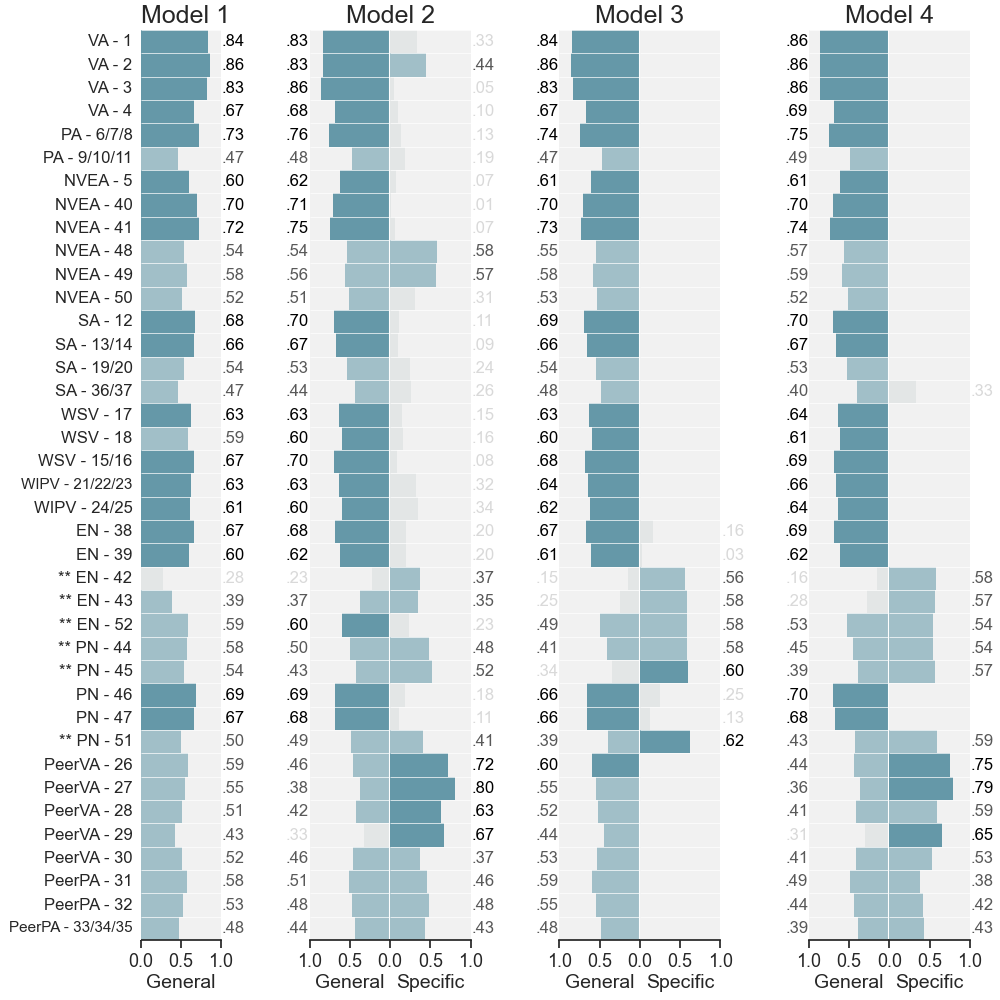
\includegraphics[width=1.1\textwidth,center]{figures/fig02.png}
    \captionsetup{width=1.1\textwidth}
    \caption{Standardized factor loadings from the four models fit to the original sample. Notes: Model 1 = one-factor (unidimensional) model; Model 2 = bifactor model with 10 specific factors; Model 3 = bifactor S-1 model with one specific factor (neglect); Model 4 = bifactor S-1 with two specific factors (peer victimization, reverse-scored); VA = verbal abuse; PA = physical abuse; NVEA = nonverbal emotional abuse; SA = sexual abuse; WSV = witnessing sibling vioence; WIPV = witnessing inter-parental violence; EN = emotional neglect; PN = physical neglect; PeerVA = peer verbal abuse; PeerPA = peer physical abuse. Factor loadings $<$ 0.3 are displayed in gray; factor loadings $\geq$ 0.6 are bolded.  ** Reverse-scored items.}
    \label{fig:loadings_original}
\end{figure}

\begin{figure}[tp]
    \centering
    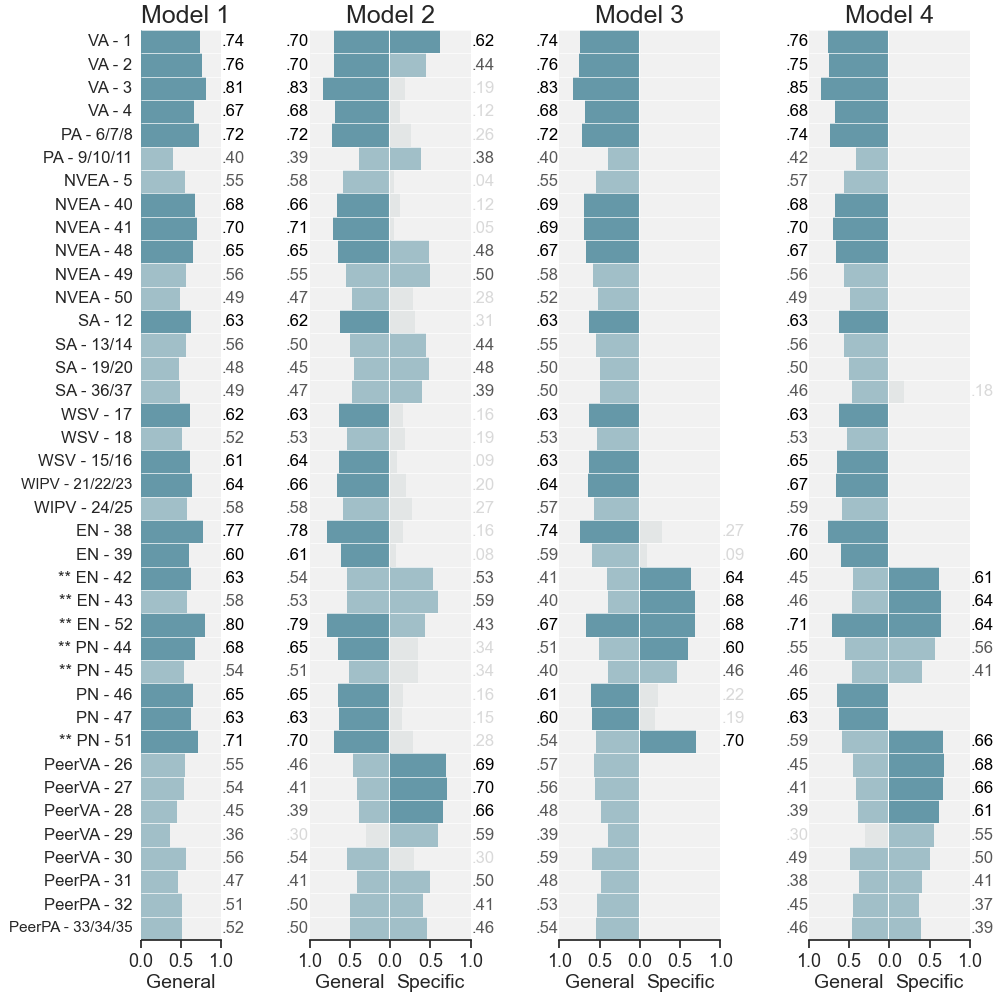
\includegraphics[width=1.1\textwidth,center]{figures/fig03.png}
    \captionsetup{width=1.1\textwidth}
    \caption{Standardized factor loadings from the four models fit to the replication sample. Notes: Model 1 = one-factor (unidimensional) model; Model 2 = bifactor model with 10 specific factors; Model 3 = bifactor S-1 model with one specific factor (neglect); Model 4 = bifactor S-1 with two specific factors (peer victimization, reverse-scored); VA = verbal abuse; PA = physical abuse; NVEA = nonverbal emotional abuse; SA = sexual abuse; WSV = witnessing sibling vioence; WIPV = witnessing inter-parental violence; EN = emotional neglect; PN = physical neglect; PeerVA = peer verbal abuse; PeerPA = peer physical abuse. Factor loadings $<$ 0.3 are displayed in gray; factor loadings $\geq$ 0.6 are bolded.  ** Reverse-scored items.}
    \label{fig:loadings_online}
\end{figure}

The item discrimination parameters of the unidimensional model were, on average, large for both the original sample (mean $\alpha$ = 1.357, 95\% HDI = 1.295 -- 1.414) and replication sample (mean $\alpha$ = 1.349, 95\% HDI = 1.272 -- 1.422). The standardized factor loadings were correspondingly large in magnitude. In the original sample, factor loadings ranged between 0.279 and 0.864 with an average value of 0.597 (95\% HDI = 0.579 -- 0.614); in the replication sample, factor loadings ranged between 0.359 and 0.814 with an average value of 0.600 (95\% HDI = 0.578 -- 0.621). Most items had loadings greater than 0.50 (original: 80.0\%, replication: 80.0\%), and therefore appear to be good indicators of general maltreatment. The rank correlation of general factor loadings between samples was $\rho$ = 0.565 (95\% HDI = 0.414 -- 0.711), indicating only moderate agreement between samples.

As an initial characterization the dimensionality of the MACE, we inspected the first six eigenvalues of the polychoric item correlation matrix for each sample. In the original sample, these values were 14.62, 3.77, 2.64, 2.11, 1.79, and 1.35; in the replication sample, they were 13.27, 4.43, 2.48, 2.04, 1.81, and 1.56. The first-to-second eigenvalue ratios of 3.84 and 3.02 are just above the 3-to-1 criterion often cited in determining whether item response data are essentially unidimensional \citep{embretson2013item}. 

In sum, the fits of the one-factor models provide partial evidence in support of a unidimensional model of the MACE. Virtually all items exhibited moderate-to-large loadings onto the common factor. Moreover, the eigenvalues of the polychoric correlation matrix suggested the presence of one primary factor. However, the degree of local dependence present among in the unidimensional model fits (especially among the peer victimization items) suggest there may be additional dimensions to the MACE. We turn next to the multidimensional confirmatory models to explore these possibilities.

\subsubsection{Model 2: Bifactor model with 10 specific factors}

Next we inspect the bifactor model with 10 specific factors, i.e. one per subscale on the MACE (model 2). In the original sample, the loadings on the general maltreatment factor ranged between 0.235 and 0.864 with an average value of 0.575 (95\% HDI = 0.556 -- 0.593). In the replication sample, the general factor loadings ranged between 0.299 and 0.827 with an average value of 0.580 (95\% HDI = 0.560 -- 0.601). The relative parameter bias was marginal for both samples (original = 2.1\%; replication = 2.7\%), suggesting there was little bias in the factor loadings of the one-factor models due to multidimensionality.  

In contrast, the loadings on the specific factors were smaller and seldom exceeded loadings on the general factor. In the original dataset, the specific factor loadings ranged between 0.014 to 0.797 with an average value of 0.313 (95\% HDI = 0.285 -- 0.341). In the replication dataset, the range was between 0.043 and 0.698, with an average value of 0.343 (95\% HDI = 0.315 -- 0.369). Only items from the two peer abuse subscales had specific factor loadings of equal or greater magnitude to those on the general factor.

\begin{table}[t!]
\centering
\begin{tabular*}{\textwidth}{crccccccccc}
\toprule
& & & \multicolumn{4}{c}{Original} & \multicolumn{4}{c}{Replication} \\
\cmidrule(lr){4-7}\cmidrule(lr){8-11}
Model & Factor & PUC & ECV & $\omega$ & $\omega_{h/s}$ & H & ECV & $\omega$ & $\omega_{h/s}$ & H \\
\midrule
2 & General &  0.912 & 0.716 &  0.963 &   0.924 &  0.964 & 0.697 & 0.965 & 0.924 & 0.961 \\
& VA        &        &       &  0.909 &   0.069 &  0.273 &       & 0.893 & 0.162 & 0.478 \\
& PA        &        &       &  0.590 &   0.037 &  0.052 &       & 0.595 & 0.148 & 0.194 \\
& NVEA      &        &       &  0.848 &   0.136 &  0.525 &       & 0.827 & 0.117 & 0.424 \\
& SA        &        &       &  0.710 &   0.059 &  0.134 &       & 0.749 & 0.290 & 0.452 \\
& EN        &        &       &  0.715 &   0.162 &  0.304 &       & 0.874 & 0.203 & 0.542 \\
& PN        &        &       &  0.800 &   0.217 &  0.479 &       & 0.812 & 0.114 & 0.284 \\
& WSV       &        &       &  0.695 &   0.027 &  0.053 &       & 0.651 & 0.037 & 0.067 \\
& WIPV      &        &       &  0.655 &   0.146 &  0.197 &       & 0.612 & 0.077 & 0.107 \\
& PeerVA    &        &       &  0.878 &   0.621 &  0.818 &       & 0.853 & 0.565 & 0.766 \\
& PeerPA    &        &       &  0.699 &   0.335 &  0.443 &       & 0.694 & 0.337 & 0.446 \\
\midrule
3 & General &  0.939 & 0.864 &  0.958 &   0.928 &  0.964 & 0.841 & 0.959 & 0.922 & 0.959 \\
& Neglect   &        &       &  0.877 &   0.384 &  0.766 &       & 0.921 & 0.375 & 0.814 \\
\midrule
4 & General &  0.931 & 0.738 &  0.961 &   0.896 &  0.965 & 0.751 & 0.961 & 0.904 & 0.960 \\
& Peer      &        &       &  0.889 &   0.569 &  0.842 &       & 0.868 & 0.493 & 0.781 \\
& Reverse   &        &       &  0.839 &   0.584 &  0.739 &       & 0.915 & 0.498 & 0.773 \\
\bottomrule
\end{tabular*}
\captionsetup{width=1.\textwidth}
\caption{\normalfont Model-based reliability indices for the three bifactor models. Notes: PUC = proportion uncontaminated correlations; ECV = explained common variance; VA = verbal abuse; PA = physical abuse; NVEA = nonverbal emotional abuse; SA = sexual abuse; EN = emotional neglect; PN = physical neglect; WSV = witnessing sibling violence; WIPV = witnessing inter-parental violence; PeerVA = peer verbal abuse; PeerPA = peer physical abuse.}
\label{table:reliability}
\end{table}

We now consider the reliability of the MACE total score. We found the MACE total score had excellent reliability (original: $\omega$ = 0.963; replication: $\omega$ = 0.965). The $\omega_h$ value was 0.924 for both samples indicating that 96.0\% and 95.8\% of the reliable variance in the total score is attributable to general maltreatment. Importantly, the ECV values were 0.716 and 0.697 for the original and replication samples, respectively. In conjunction with a PUC value of 0.912, the ECV values suggest the MACE is essentially unidimensional despite the multidimensionality of its contents. Together, the results support the interpretation of the MACE total score is a reliable and valid measure of overall maltreatment.

Next we consider the reliability of the MACE subscale scores, where the results are in direct contrast to the MACE total score. As would be expected given the lower number of items, the reliability of the subscales was both lower and more variable. The $\omega$ values ranged between 0.590 and 0.909 in the original sample, and between 0.595 and 0.893 in the replication sample. Most subscale scores exhibited at least adequate reliability (>0.7). Crucially, subscale scores for both samples contained little reliable variance after controlling for the general maltreatment factor (original: mean $\omega_s$ = 0.181, range = 0.027 -- 0.621; replication: mean $\omega_s$ = 0.205, range = 0.037 -- 0.565). That is, the reliability of MACE subscale scores primarily reflect general maltreatment and not any specific type of maltreatment. The only exception was for the peer verbal abuse subscale, where more than half the reliable variance in subscale scores was independent of general maltreatment (original = 70.7\%; replication = 66.2\%).

To summarize, the results of the full bifactor model (model 2) indicate responses on the MACE are explained by a dominant general maltreatment factor characterized by large loadings across items. In contrast, specific factors representing each MACE subscale are characterized by mostly small factor loadings that contribute little reliable variance to total and subscale scores. Where the MACE total score is a reliable and valid measure of overall maltreatment, the majority of MACE subscale scores contain little reliable variance unique from general maltreatment. Therefore, they should not be interpreted as reflecting specific types of maltreatment. One question that remains, however, is if other reliable subscale scores can be derived from the MACE. 

\subsubsection{Model 3: Bifactor S-1 model with one specific factor (neglect)}

We turn our attention next to the bifactor S-1 model with one specific factor (neglect; model 3). The loadings on the general factor largely resembled those of the bifactor model. In the original sample, the loadings on the general maltreatment factor ranged between 0.150 and 0.864 with an average value of 0.577 (95\% HDI = 0.558 -- 0.594). In the replication sample, the general factor loadings ranged between 0.395 and 0.831 with an average value of 0.580 (95\% HDI = 0.558 -- 0.601). 

The loadings on the neglect specific factor were smaller on average. In the original sample, the average specific loading was 0.410 (95\% HDI = 0.373 -- 0.454); in the replication sample, it was 0.454 (95\% HDI = 0.409 -- 0.499). The specific loadings displayed a troubling pattern where only the six reverse-scored items exhibited moderate loadings on the specific factor; the remaining four item exhibited negligible factor loadings. That is, the ``neglect'' factor appears instead to reflect a reverse-scored methods factor.

Moving on to the reliability measures, we again found that the total score exhibited excellent reliability (original: $\omega$ = 0.958; replication: $\omega$ = 0.959). Moreover, the $\omega_h$ values indicated the majority of reliable variance in severity score was attributable to the general factor (original: $\omega_h$ = 0.928; replication: $\omega_h$ = 0.922). The reliability of the ``neglect'' subscale score was also good (original: $\omega$ = 0.877; replication: $\omega$ = 0.921). As indicated by the $\omega_s$ values, however, reliable variance in the ``neglect'' subscale scores primarily reflected the general maltreatment factor (original: $\omega_h$ = 0.384; replication: $\omega_h$ = 0.375). 

In sum, the results do not support the use of the MACE to compute separate threat and neglect subscale scores. The neglect subscale scores posses an unsatisfactory amount of reliable variance unique from general maltreatment; therefore, they cannot be interpreted as meaningfully reflecting neglect. Furthermore, the majority of items measuring neglect on the MACE seem to be contaminated by a reverse-scored methods factor.

\subsubsection{Model 4: Bifactor S-1 with two specific factors (peer victimization, reverse- scoring)}

Finally, we turn to the bifactor S-1 model with two specific factors (peer victimization, reverse-scoring; model 4). In the original sample, the loadings on the general maltreatment factor ranged between 0.158 and 0.864 with an average value of 0.563 (95\% HDI = 0.545 -- 0.580). In the replication sample, the general factor loadings ranged between 0.298 and 0.852 with an average value of 0.572 (95\% HDI = 0.550 -- 0.593). Interestingly, the loadings on the specific factors were of approximately equal magnitude. In the original dataset, the specific factor loadings ranged 0.327 to 0.789 with an average value of 0.550 (95\% HDI = 0.522 -- 0.576). In the replication dataset, the range was between 0.183 and 0.684 with an average value of 0.526 (95\% HDI = 0.492 -- 0.556). 

As before, the MACE total score again exhibited excellent reliability (original: $\omega$ = 0.961; replication: $\omega$ = 0.961). Similarly, the majority of reliable variance in severity score was attributable to the general factor (original: $\omega_h$ = 0.896; replication: $\omega_h$ = 0.904). The peer victimization subscale scores exhibited good reliability across samples (original: $\omega$ = 0.889; replication: $\omega$ = 0.868). The corresponding $\omega_s$ values were 0.569 for the original sample and 0.493 for the replication sample indicating that slightly more than half of the variance in peer victimization scores were independent of the general maltreatment factor (original: 64.0\%; replication: 56.8\%). Thus, the results suggest (albeit weakly so) the presence a secondary peer victimization factor in the MACE in addition to the general maltreatment factor. 

Briefly, we note that the subscale scores formed by the reverse-scored items were also reliable (original: $\omega$ = 0.839; replication: $\omega$ = 0.915). Moreover, the corresponding $\omega_s$ values were similar in magnitude to those observed for the peer victimization scores (original: $\omega_s$ = 0.584; replication: $\omega_s$ = 0.498). In other words, these scores also exhibit majority reliable variance unique from general maltreatment. It is difficult to interpret these scores, however, as it is unclear what they primarily reflect (e.g. neglect, wording effects, and/or scoring-induced methods artifact). 

\section{Discussion}

The MACE is a promising measure of childhood maltreatment \citep{georgieva2022systematic}. Despite its increasing popularity, there has been little investigation of its structural validity \citep{saini2019systematic}, leaving unanswered questions about its factor structure and the interpretation of its total \& subscale scores. Here we investigated the factor structure of the MACE, using a series confirmatory item response models, in two independent samples. The primary goal of our analyses was to evaluate the reliability of the MACE total and subscale scores, and to determine whether the latter would provide unique information above and beyond the total score. A secondary goal was to examine the dimensionality of the MACE; that is, whether its inter-item covariance was best-explained by a hierarchical structure with 10 factors (one per subscale) or by a more parsimonious structure. 

Regarding our first goal, we found the MACE total score has excellent reliability and overwhelmingly reflects general maltreatment. That is, despite being a composite of items measuring 10 distinct types of maltreatment, the MACE total score is a univocal index of overall childhood maltreatment. In stark contrast, although we found the MACE subscale scores exhibited adequate reliability on average, we also found that these scores mostly reflected general maltreatment and not any particular type of maltreatment as intended. The same was true of neglect subscale scores (composed of the physical and emotional neglect subscales), which were additionally contaminated by a reverse-scored methods factor. In short, our results support the continued use of the MACE total score but caution against the use of MACE subscale scores. Indeed the latter have little practical use given the low reliability of the portion of subscale scores independent of the total score.

Regarding our second goal, confirmatory bifactor models of the MACE revealed a dominant general maltreatment factor, characterized by uniformly strong loadings across items, and much weaker specific factors. Importantly, general factor loadings from the bifactor models strongly resembled their corresponding loadings from a one-factor model. Moreover, the general factor explained approximately 70\% of the reliable variance in participants' responses. Together, these results support the conclusion that, while the item content of the MACE is multidimensional, its factor structure is essentially unidimensional. In other words, researchers can safely interpret the MACE total score as an index of overall maltreatment; they can also expect little bias in factor loading estimates if they were to specify a one-factor model to explain responses on the MACE. 

Of the four confirmatory factor models we tested, the most parsimonious and best- fitting was a bifactor S-1 model with a general maltreatment factor and two specific factors measuring peer victimization and reverse-scoring. This model provided a fit to the response data as good as the more complex full bifactor model with 10 specific factors. (This bifactor S-1 model was also partially supported by exploratory factor analyses; see the supplement for details.) Thus, our results suggest the factor structure of the MACE is essentially unidimensional with two secondary factors affecting a subset of items. Notably, we found that the scores from the peer victimization subscale (composed of items from the peer physical and emotional abuse subscales) were viable. That is, they were reliable and, after controlling for general maltreatment, a majority of their reliable variance was attributable to peer victimization. Researchers may therefore be justified in using peer victimization subscale scores from the MACE, but additional research is needed to validate this index.

Our results are consistent with a number of previous studies investigating the factor structure of other childhood maltreatment questionnaires. For example, bifactor models of the Childhood Trauma Questionnaire have also revealed a dominant general maltreatment factor and weaker specific factors \citep{spinhoven2014childhood, stagaki2022mediating}. Similar results were found in recent applications of a bifactor model to the International Child Abuse Screening Tool \citep{meinck2021factor} and the Adverse Childhood Experience questionnaire \citep{dobson2021latent}. Together, these and our current results underscore a challenge in investigating the consequences of childhood maltreatment: when maltreatment experiences tend to co-occur, it is difficult to measure the effects of a particular type of adversity unique from overall maltreatment.  
 
Our results are also worth considering alongside previous studies that used MACE subscale scores to investigate the link between particular types of childhood maltreatment and assorted psychobiological outcomes. For example, researchers have looked at the relationship between MACE subscale scores and risk of depression \citep{gerke2018childhood}, dissociative symptoms, \citep{schalinski2015type}, and cortisol concentration \citep{schalinski2019early}. Still others have used threat and deprivation subscale scores from the MACE to study their associations with cognitive functioning \citep{schalinski2018defining} and hippocampal volume \citep{teicher2018differential}. Our results are clear that these scores chiefly reflect general maltreatment and not particular types of adversity, which presents a challenge for interpreting the conclusions of those studies. It is worth noting that some of these studies attempted to control for general maltreatment by entering all of the MACE subscale scores simultaneously into sophisticated multivariate analyses (e.g. random forest regression). This approach is unsatisfactory for two reasons. First, random forest models can produce spurious results when given collinear predictors \citep{gregorutti2017correlation}. Second, even if one were to properly control for general maltreatment, our results indicate that the remaining reliable variance in most subscale scores would be so low as to cause doubt about the meaning of any subsequent inferences.

The current study revealed other features of the MACE worth highlighting. For example, we identified several sources of DIF in the MACE. We found that across samples women experienced more sexual abuse whereas men experienced more physical abuse by peers. These findings are in line with previous research \citep{radford2013prevalence}. We also identified a number of items with DIF by sample. The cause for this is unclear and may reflect differences in sample population (greater Boston area vs. US \& Canada), study location (in clinic vs. online), recruitment years (early 2010s vs. early 2020s), inclusion criteria (healthy \& unmedicated vs. none), and/or exclusion criteria (none vs. attention checks). The causes and impact of violations of measurement invariance on the MACE require further study. 

We also identified a reverse-scored methods factor in the MACE. In our view, the most plausible explanation is that, under the \cite{teicher2015maltreatment} scoring procedure, affirmative responses on the regular and reverse-scored items on the MACE represent very different endorsements. For a regular item on the MACE, an endorsement indicates that a person experienced an adverse event during one year of childhood at least. In contrast, an endorsement on a reverse-scored item indicates that a person experienced experienced the absence of a positive event for all 18 years of childhood. However, alternative causes of the reverse-scored factor (e.g. participant confusion, acquiescence, or carelessness; \citealt{weijters2013reversed}) are possible. Additional research is needed to see if alternative scoring procedures would eliminate this factor. 

The current study is not without limitations. The most apparent limitation is that we only studied the dichotomous response data, but not the chronology data that is also collected as part of the MACE. Though we found that the factor structure of the endorsement responses is essentially unidimensional, this may belie more complex patterns present in the maltreatment chronology data. Indeed, longitudinal models of adverse events across childhood --- perhaps using dynamic factor analysis \citep{zhang2007bayesian} --- might be more sensitive to patterns of maltreatment covariation that are lost when collapsing the data into a dichotomous indicator of none vs. any maltreatment. Another possibility is to jointly model the MACE endorsement and chronology data using a multidimensional hurdle model \citep{magnus2021symptom}, which measures both a person's susceptibility to maltreatment (number of maltreatment experiences) and severity of maltreatment (duration of maltreatment experiences). Further research is needed to develop maltreatment scores that integrate the MACE endorsement and chronology data. 

A second limitation is our sample demographics. Though the replication sample increased the overall diversity of our sample with respect to gender and age, other types of diversity are notably lacking. Our combined sample was neither racially nor ethnically diverse. This is important as previous studies have identified DIF for childhood adversity questionnaires by race \citep{rodriguez2019identification}, which raises the question whether similar issues would be found for the MACE in more diverse samples. Moreover, we are not currently able to explain why we found DIF in multiple items by sample membership in the current study. Additional research is needed to study the functioning of the MACE in more diverse samples in order to validate its use in different populations. 

To conclude, the results of the current study show the factor structure of the MACE is essentially unidimensional. Bifactor models revealed that, despite the presence of smaller secondary factors, the majority of reliable variance in the MACE endorsement responses are attributable to a general maltreatment factor. Accordingly, we found that the MACE total score is a reliable and valid measure of overall childhood maltreatment. In contrast, we found that MACE subscale scores are unreliable measures of their intended constructs; that is, they primarily reflect general maltreatment and not any specific type of maltreatment. Moving forward, childhood maltreatment researchers using the MACE (or any other scale) should be careful to ensure that any total or subscale scores they use as part of their analyses are reliable, lest they risk drawing spurious inferences. 

\bibliography{main}

\pagebreak
\section{Supplementary materials}

\setcounter{figure}{0}
\setcounter{table}{0}
\renewcommand{\thetable}{S\arabic{table}}
\renewcommand{\thefigure}{S\arabic{figure}}

\subsection*{Reflective vs. formative indicator models of maltreatment data}

One might question whether it is appropriate to explain childhood maltreatment data using common factor models with reflective indicators (e.g. bifactor models). The core assumption of these models is that variation in item responses are caused by or reflect variation in a shared latent factor (e.g. variation in low mood and anergia reflect latent individual differences in depression). This is in contrast to composite variable models with formative indicators where the direction of causality is reversed \citepSM{bollen1991conventional}. In composite variable models, indicators cause or form the latent construct (e.g. education and income together make up socioeconomic status). Some scholars have argued that measures of adverse childhood experiences should often be treated as formative, not reflective, indicators \citepSM{netland2001assessment, layne2010unpacking}. That is, exposure to abuse and neglect defines childhood maltreatment, not the other way around. 

For the purposes of explaining covariation in participants' responses on the MACE, we believe we are justified in using a common factor model. Most of the items on the MACE measure maltreatment by parents or other guardians. The homogeneity of these indicators suggests they might reflect a common source --- a hypothesis that is further supported by the uniformly strong (general) factor loadings we observed for this subset of items. Furthermore, there is ample theoretical and empirical support for regarding parental maltreatment as a common factor with its own causal antecedents \citepSM{belsky1993etiology}. Indeed, many of the same parent-level variables (e.g. emotional lability, impulse control, own history of abuse) are risk factors for different types of childhood maltreatment \citepSM{stith2009risk, mulder2018risk, assink2019risk}. 

Separately, that the MACE is a retrospective self-report measure is further justification for a common factor model. Retrospective measures of abuse have been shown to reflect additional factors beyond exposure to maltreatment including individual differences in current emotional state, personality, and recall ability \citepSM{susser2012still, reuben2016lest, colman2016consistency}. Common factor models are better suited to adjust the measurement error in indicators caused in part by these nuisance factors.

This discussion in turn raises a second question: is it reasonable for the items measuring parental maltreatment and peer victimization on the MACE to share a common factor? One might assume that these two types of maltreatment reflect independent causes and should therefore not be permitted to share a common factor. There is considerable evidence, however, that children who have been maltreated are at greater risk for subsequent peer victimization \citepSM{bolger2001developmental, benedini2016cycle}. The reasons for this association are manifold. For example, parental maltreatment may impact a child's sociocognitive functioning (e.g. attachment styles, emotion regulation) in ways that may predispose them to later peer victimization \citepSM{goemans2021child, McCrory2022-cj}. Separately, parental neglect is a risk factor for peer victimization \citepSM{lereya2013parenting}, possibly by increasing the chance that children enter into risky social situations where victimization may occur. Insofar that parental maltreatment is an indirect cause of peer victimization (mediated by multiple complex psychosocial pathways), then we believe we are justified in allowing indicators of peer victimization to load onto the common general maltreatment factor. This is also highlights the need for future study of MACE peer victimization subscale scores in order to better understand how it is similar to (and distinct from) parental maltreatment, and what their downstream sequalae are. 

\subsection*{Additional self-report measures}

In addition to the MACE, participants in both samples completed a number of additional self-report measures. Participants in the original sample completed multiple measures concerning psychiatric symptoms; these have already been reported \citepSM{teicher2015maltreatment}. The participants in the replication sample completed three additional self-report measures assessing negative symptoms and motivation for rewards. Specifically, participants completed the Motivation and Pleasure scale \citepSM{llerena2013motivation}, the Self-evaluation of Negative Symptoms scale \citepSM{dollfus2016self}, and the revised Behavioral Inhibition / Behavioral Activation scale \citepSM{pagliaccio2016revising}.

Following best practices for online research \citepSM{zorowitz2021inattentive}, several attention checks were embedded in the secondary self-report measures filled out by the replication sample. Specifically, we used infrequency items which are questions for which all  or virtually all attentive participants should provide the same response. Specifically, we used the following questions:

\begin{enumerate}
    \item I'm able to blink my eyes without difficulty. (all endorse)
    \item I was motivated to write Mumfred Mumford's biography. (none endorse)
    \item I worry about the 2001 Cricket World Cup. (none endorse)
    \item Please select ``Yes'' and then select age ``17''. (instructed item)
\end{enumerate}

\noindent Prior to conducting the study, the infrequency items were piloted on an independent sample of participants to ensure that they elicited one dominant response. Participants were excluded from analysis if they responded incorrectly to one or more of these items.

\subsection{Exploratory factor analysis}

In addition to confirmatory factor analysis, we also performed exploratory factor analysis (EFA) on the response data from each sample separately. The goal of the EFA was to examine what factor structure would emerge with no \emph{a priori} restrictions placed on the data. We decided to extract two- and three- factor solutions based on the total number of factors in the bifactor S-1 models. We were particularly interested to see if a two-factor solution would reproduce the factors from model 3 (threat, deprivation); and if a three- factor solution would reproduce the three factors from model 4 (parental maltreatment, peer victimization, reverse-scored). 

EFA was performed using the \textit{lavaan} (v0.6.11; \citealt{lavaan}) package available in R. Factors were extracted using the oblique geomin \citep{yates1987multivariate} and cf-quartimax rotation criteria \citep{crawford1970general}, which were selected in order to extract simple factor structures with few cross-loadings. We used two rotation criteria in order to examine the generalizability of the factor solutions across rotations. We again relied on traditional fit indices (i.e. RMSEA, CFI, TLI) to evaluate the goodness-of-fit of the exploratory factor models to the response data of both samples.

The goodness-of-fit measures for the exploratory factor models to the response data by sample are summarized in Table \ref{tab:efa_diagnostics}. The fit indices indicated that all exploratory models provided adequate fits to the data. The standardized factor loadings for the 2- and 3-factor solutions produced by the cf-quartimax rotation are presented in Figure \ref{fig:efa_cf}. The corresponding factor loadings produced by the geomin rotation were qualitatively similar and are presented in Figure \ref{fig:efa_geomin}. In the 2-factor solution for the original sample, we observed a primary parental maltreatment factor and a secondary peer victimization factor. In contrast, the replication sample produced an unclear factor solution characterized by strong loadings from the everse-scored items (F1) and peer victimization (F2). The parental maltreatment items then weakly loaded on both factors. Neither 2-factor solution precisely resembled the threat-deprivation factor structure of confirmatory model 3.

The 3-factor solutions for each sample were similar. EFA produced a primary parental maltreatment factor with secondary peer victimization and reverse-scored factors. Interestingly, items concerning sexual abuse loaded less strongly on the parental maltreatment factor in the replication sample, raising some questions about the replicability of the factor structures. Nevertheless, the structure of both the 2- and 3-factor exploratory factor models resembled most closely the bifactor S-1 model with two specific factors (model 4), providing further support for that model of the factor structure of the MACE. 

\pagebreak
\subsection*{Supplementary tables \& figures}

\begin{longtable}{P{0.02\linewidth}p{0.7\linewidth}|P{0.05\linewidth}P{0.05\linewidth}P{0.05\linewidth}}
\centering
\# & Item & \multicolumn{3}{c}{Tetrachoric Corr.} \\
\toprule
6 & {\small Intentionally pushed, grabbed, shoved, slapped, pinched, punched or kicked you.} & - & & \\
7 & {\small Hit you so hard that it left marks for more than a few minutes.} & 0.778 & - &  \\
8 & {\small Hit you so hard, or intentionally harmed you in some way, that you received or should have received medical attention.} & 0.702 & 0.758 & - \\
\midrule
9& {\small Spanked you on your buttocks, arms or legs.} & - & \\
10	& {\small Spanked you on your bare (unclothed) buttocks.} & 0.862 & - & \\
11 & {\small Spanked you with an object such as a strap, belt, brush, paddle, rod, etc.} & 0.816 & 0.519 & - \\
\midrule
13 & {\small Touched or fondled your body in a sexual way.} & - \\
14 & {\small Had you touch their body in a sexual way.} & 0.954 & - \\
\midrule
15 & {\small Hit your sibling (stepsibling) so hard that it left marks for more than a few minutes.} &  \\
16 & {\small Hit your sibling (stepsibling) so hard, or intentionally harmed him or her in some way, that he/she received or should have received medical attention.} & 0.966 & - \\
\midrule
19 & {\small Had you touch their body in a sexual way.} & - \\
20 & {\small Actually had sexual intercourse (oral, anal or vaginal) with you.} & 0.909 & - \\
\midrule
21 & {\small Saw adults living in the household push, grab, slap or throw something at your mother (stepmother, grandmother).} & - \\
22 & {\small Saw adults living in the household hit your mother, stepmother, or grandmother so hard that it left marks for more than a few minutes.} & 0.920 & -  \\
23 & {\small Saw adults living in the household hit your mother, stepmother, or grandmother so hard, or intentionally harm her in some way, that she received or should have received medical attention.} & 0.808 & 0.934 & - \\
\midrule
24 & {\small Saw adults living in the household push, grab, slap or throw something at your father (stepfather, grandfather).} &  \\
25 & {\small Saw adults living in the household hit your father, stepfather, or grandfather so hard that it left marks for more than a few minutes.} & 0.900 & -\\
\midrule
33 & {\small Peers intentionally pushed, grabbed, shoved, slapped, pinched, punched, or kicked you.} & - \\
34 & {\small Peers hit you so hard that it left marks for more than a few minutes.} & 0.829 & - \\
35 & {\small Peers hit you so hard, or intentionally harmed you in some way, that you received or should have received medical attention.} & 0.723 & 0.907 & - \\
\midrule
36 & {\small Peers forced you to engage in sexual activity against your will.} &  - & \\
37 & {\small Peers forced you to do things sexually that you did not want to do.} & 0.975 & - \\
\bottomrule
\caption{\normalfont The 12 item pairs and triplets in the MACE characterized by response dependence. The tetrachoric correlation (averaged over samples) for each pair of items in a set is presented in tandem with the item wording.}
\label{tab:dependence}
\end{longtable}

\begin{table}[H]
    \centering
    \begin{tabular}{llccccc}
    \toprule
    Sample      & Model    & $\chi^2$ ($df$) & RMSEA & CFI & TLI & SRMR \\
    \midrule
    Original    & 2-factor & 1876 (664) & 0.049 & 0.962 & 0.957 & 0.122 \\
                & 3-factor & 1237 (627) & 0.036 & 0.981 & 0.977 & 0.105 \\
    \midrule
    Replication & 2-factor & 1612 (664) & 0.051 & 0.961 & 0.957 & 0.121 \\
                & 3-factor & 1100 (627) & 0.037 & 0.981 & 0.977 & 0.111 \\
    \bottomrule
    \end{tabular}
    \caption{\normalfont Fit statistics for the exploratory factor models by sample. Notes: RMSEA = root mean square error of approximation; CFI = comparative fit index; TLI = Tucker-Lewis index; SRMR = standardized root mean square residual.}
    \label{tab:efa_diagnostics}
\end{table}

\begin{figure}[H]
    \centering
    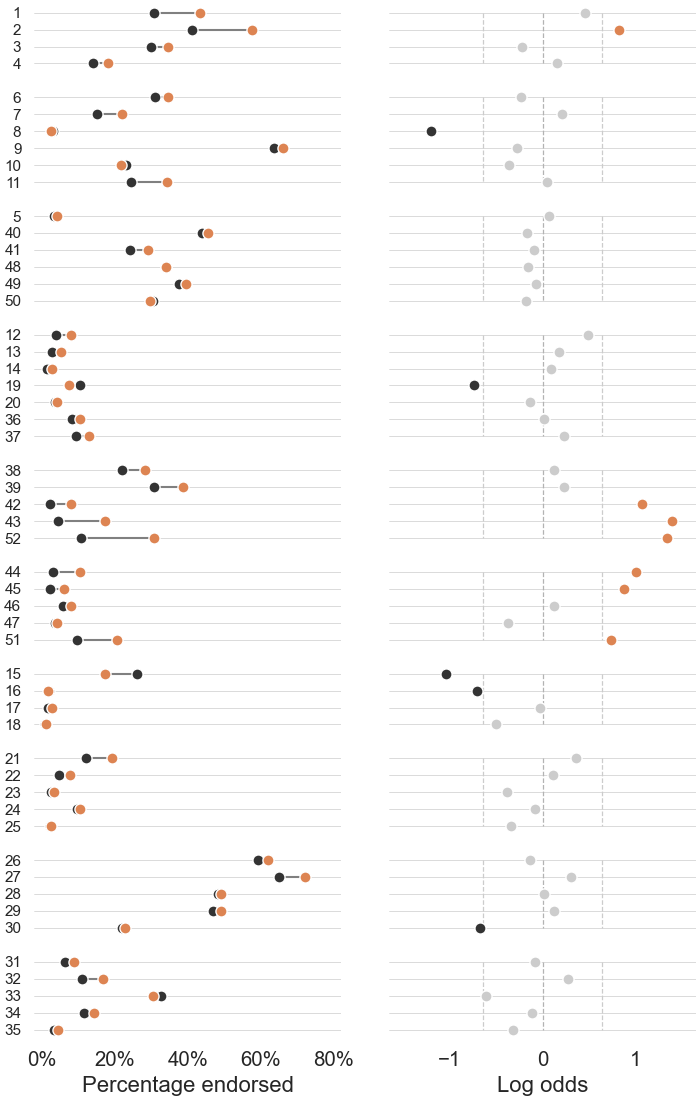
\includegraphics[width=0.82\textwidth,center]{figures/figS01.png}
    \caption{\normalfont Differential item functioning by sample. (A) Proportions of participants endorsing having experienced a maltreatment event by study sample. (B) The log odds that the proportion of endorsements are larger in one or the other sample. Dotted lines indicate the threshold for large DIF recommended by \cite{hidalgo2014binary}. ** Reverse-scored items.}
    \label{fig:dif_study}
\end{figure}

\begin{figure}[H]
    \centering
    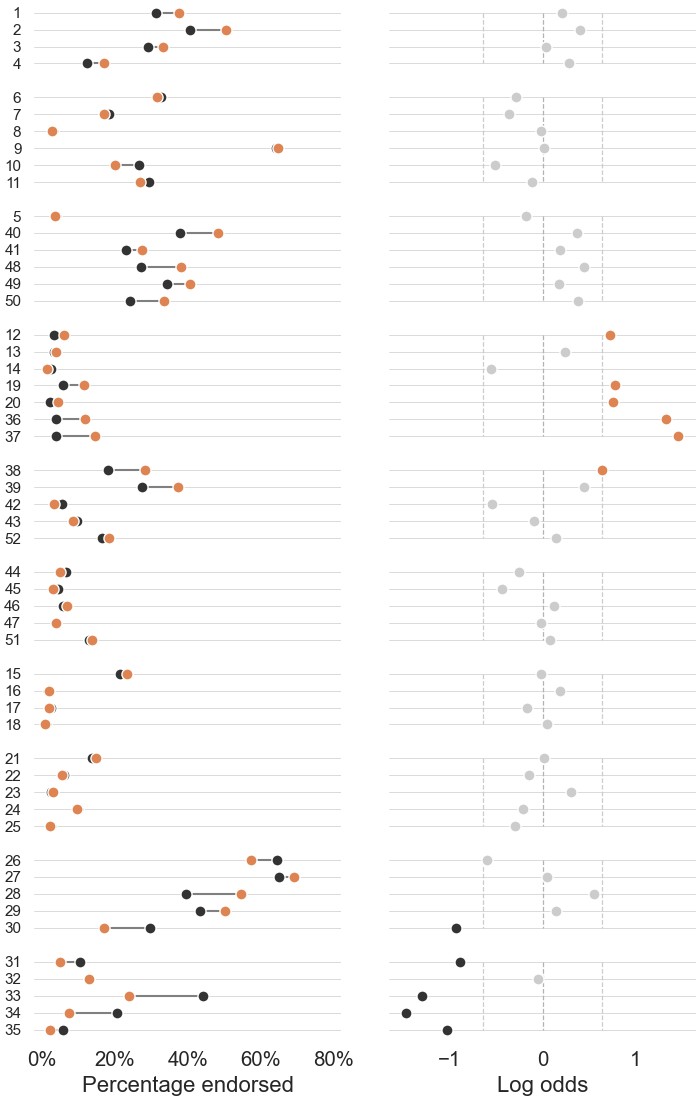
\includegraphics[width=0.82\textwidth,center]{figures/figS02.png}
    \caption{\normalfont Differential item functioning by gender. (A) Proportions of participants endorsing having experienced a maltreatment event by study gender. (B) The log odds that the proportion of endorsements are larger in one or the other gender. Dotted lines indicate the threshold for large DIF recommended by \cite{hidalgo2014binary}. ** Reverse-scored items.}
    \label{fig:dif_gender}
\end{figure}

\begin{figure}[H]
    \centering
    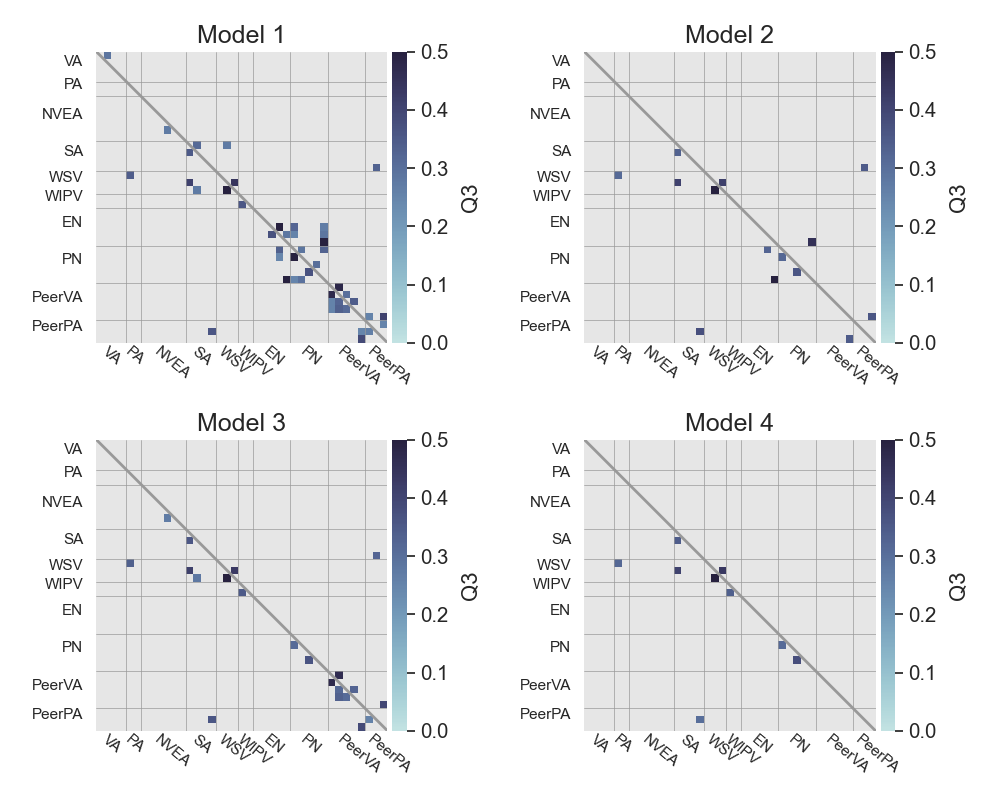
\includegraphics[width=1.05\textwidth,center]{figures/figS03.png}
    \caption{\normalfont Yen's $Q_3$ values for item pairs exceeding the 99\% percentile critical value for each confirmatory item response model. Cells beneath the gray diagonal line correspond to the original sample, whereas cells above the line correspond to the replication sample. Notes: VA = verbal abuse; PA = physical abuse; NVEA = nonverbal emotional abuse; SA = sexual abuse; EN = emotional neglect; PN = physical neglect; WSV = witnessing sibling violence; WIPV = witnessing inter-parental violence; PeerVA = peer verbal abuse; PeerPA = peer physical abuse.}
    \label{fig:local_dependence}
\end{figure}

\begin{figure}[H]
    \centering
    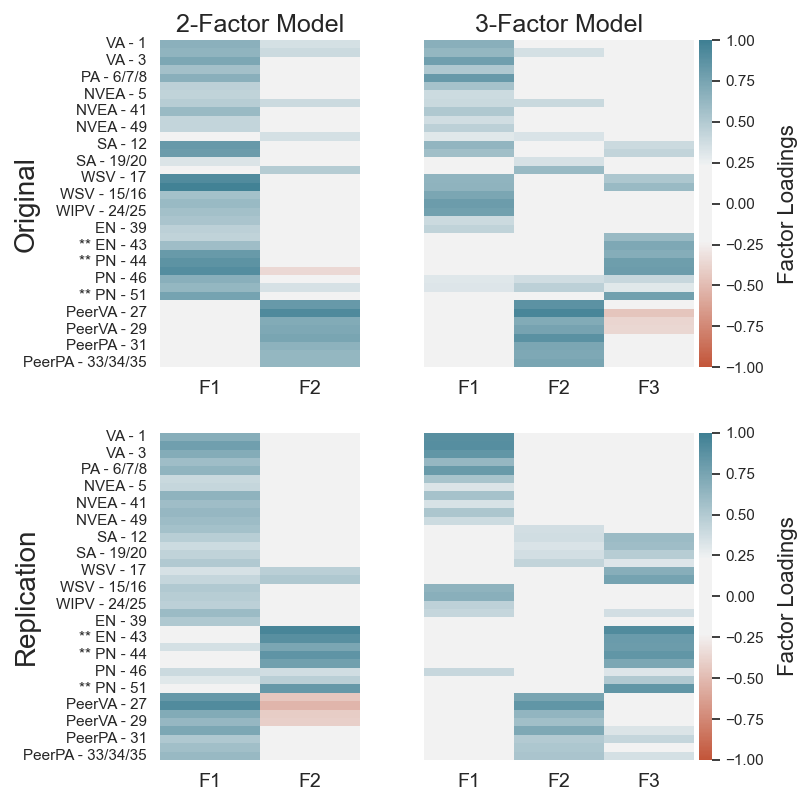
\includegraphics[width=1\textwidth,center]{figures/figS04.png}
    \caption{\normalfont Standardized factor loadings for the 2- and 3-factor solutions produced by the cf-quartimax rotation for original sample (top row) and replication sample (bottom row). \break \small Notes: VA = verbal abuse; PA = physical abuse; NVEA = nonverbal emotional abuse; SA = sexual abuse; EN = emotional neglect; PN = physical neglect; WSV = witnessing sibling violence; WIPV = witnessing inter-parental violence; PeerVA = peer verbal abuse; PeerPA = peer physical abuse. Only factor loadings $\geq$ 0.30 are shown. ** Reverse-scored items.}
    \label{fig:efa_cf}
\end{figure}

\begin{figure}[H]
    \centering
    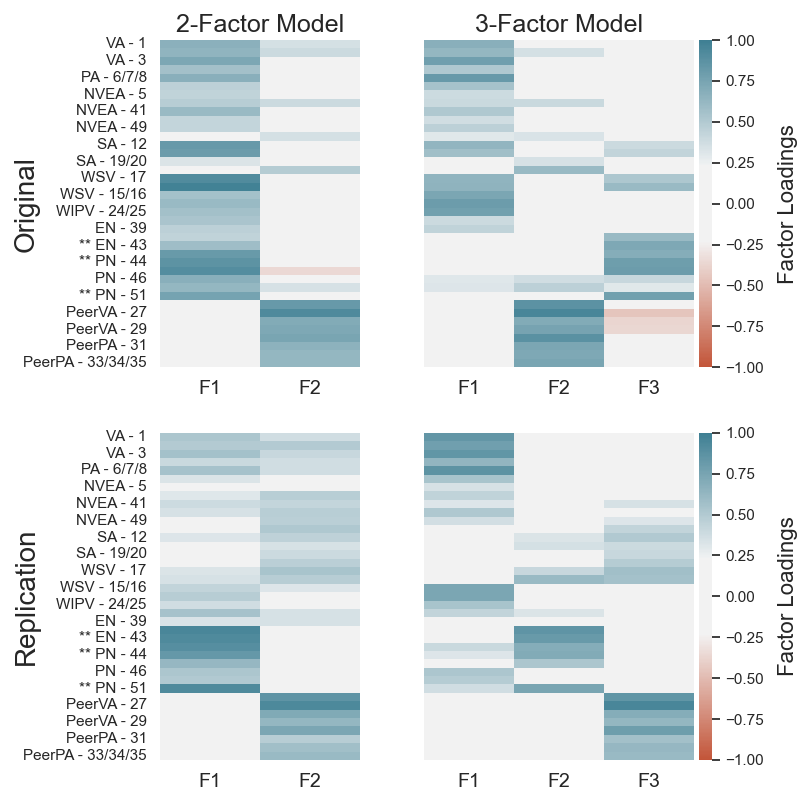
\includegraphics[width=1\textwidth,center]{figures/figS05.png}
    \caption{\normalfont Standardized factor loadings for the 2- and 3-factor solutions produced by the geomin rotation for original sample (top row) and replication sample (bottom row). Notes: VA = verbal abuse; PA = physical abuse; NVEA = nonverbal emotional abuse; SA = sexual abuse; EN = emotional neglect; PN = physical neglect; WSV = witnessing sibling violence; WIPV = witnessing inter-parental violence; PeerVA = peer verbal abuse; PeerPA = peer physical abuse. Only factor loadings $\geq$ 0.30 are shown. ** Reverse-scored items.}
    \label{fig:efa_geomin}
\end{figure}

\bibliographystyleSM{apalike}
\bibliographySM{main}

\end{document}
